\documentclass{eptcs}
\providecommand{\event}{Mieke Massink and Gethin Norman (Eds.):
Ninth Workshop on Quantitative Aspects of Programming Languages (QAPL 2011)} \providecommand{\volume}{??} \providecommand{\anno}{2011}
\providecommand{\firstpage}{1} \providecommand{\eid}{??}
\usepackage{breakurl}        
\usepackage{graphicx}
\usepackage{color}
\usepackage{epsfig}
\usepackage{amssymb}
\usepackage{amsmath}
\usepackage{amsthm}
\usepackage[ansinew]{inputenc}
\usepackage{dsfont}
\usepackage{fancybox,tikz}

\newtheorem{theorem}{Theorem}
\newtheorem{lemma}{Lemma}
\newtheorem{proposition}{Proposition}
\newtheorem{definition}{Definition}
\newtheorem{corollary}{Corollary}
\newtheorem{example}{Example}
\newtheorem{remark}{Remark}

\title{Time Delays in Membrane Systems and Petri Nets}
\author{Bogdan Aman
\institute{A.I.Cuza University\\
Blvd. Carol I, no.11, 700506 Ia\c si, Romania}
\email{bogdan.aman@gmail.com}
\and Gabriel Ciobanu
\institute{Institute of Computer Science, Romanian Academy\\
and ''A.I.~Cuza'' University of Ia\c si, Romania}
\email{gabriel@info.uaic.ro} }
\def\titlerunning{Time Delays in Membrane Systems and Petri Nets}
\def\authorrunning{B. Aman and G. Ciobanu}
\begin{document}
\maketitle

\begin{abstract}

Timing aspects in formalisms with explicit resources and parallelism are
investigated, and it is presented a formal link between timed membrane systems
and timed Petri nets with localities. For both formalisms, timing does not
increase the expressive power; however both timed membrane systems and timed
Petri nets are more flexible in describing molecular phenomena where time is a
critical resource. We establish a link between timed membrane systems and timed
Petri nets with localities, and prove an operational correspondence between
them.

\end{abstract}

\section{Introduction}
\label{section:introduction}

The evolution of complex real systems frequently involves various
interactions among components. Some mathematical models of such systems
combine both discrete and continuous evolutions on multiple time scales
with many orders of magnitude. For example, the molecular operations of a
living cell can be thought of as such a dynamical system. The molecular
operations happen on time scales ranging from  to  seconds,
and proceed in ways which are dependent on populations of molecules ranging
in size from as few as approximately  to approximately as many as
. Molecular biologists have used formalisms developed in computer
science (e.g. hybrid Petri nets) to get simplified models of some molecular
phenomena like transcription and gene regulation processes. According to
molecular cell biology \cite{Lodish08}:
(i) ``the life span of intracellular proteins varies from as
short as a few minutes for mitotic cycles, which help regulate
passage through mitosis, to as long as the age of an organism for
proteins in the lens of the eye'', and
(ii) ``Most cells in multicellular organisms  carry
out a specific set of functions over periods of days to months or
even the lifetime of the organism (nerve cells, for example)''.
Lifetimes play an important role in the
biological evolution; we mention an example from the immune system.
\begin{example}
According to \cite{Lodish08}, T-cell precursors arriving in the thymus from
the bone marrow spend up to a week differentiating there before they enter
a phase of intense proliferation. In a young adult mouse the thymus
contains around  to  thymocytes. About 
new cells are generated each day; however, only about  to  (roughly ) of these will leave the thymus each day as mature T
cells. Despite the disparity between the numbers of T cells generated daily
in the thymus and the number leaving, the thymus does not continue to grow
in size or cell number. This is because approximately  of the
thymocytes which develop in the thymus also die within the thymus.
\end{example}

Among the formalisms able to model these systems by using explicit
resources, parallelism and timing, we refer to membrane systems
\cite{Paun02} and Petri nets \cite{Jensen92,Peterson81}. Membrane
systems were extended with timing aspects in
\cite{Cavaliere05,Cavaliere10}. Petri Nets have two main extensions
with time: Time Petri Nets \cite{Merlin74} (a transition can fire
within a time interval) and Timed Petri Nets \cite{Ramchandani74} (a
transition fires as soon as possible). In Petri nets, time
can be considered relative both to places and transitions
\cite{Pezze99,Sifakis80}. In this paper, we define a timed extension
(relative to transitions) for Petri nets with localities, and we
establish a link between timed membrane systems and timed Petri nets
with localities.

Some connections between membrane systems and Petri nets are presented for the
first time in \cite{Zilio04,Qi04}. A direct structural relationship between
these two formalisms is established in \cite{Kleijn10,Kleijn06} by defining a
new class of Petri nets called Petri nets with localities. Localities are used
to model the regions of membrane systems. This new class of Petri
nets has been used to show how maximal evolutions from membrane systems are
faithfully reflected in the maximally concurrent step sequence semantics of
their corresponding Petri nets with localities.

Despite the fact that various timed extensions exist for both
membrane systems and Petri nets, we are not aware of any connection
between these timed extensions. Thus, we relate timed membrane
systems with timed Petri nets with localities. The existing links
(marked by citation or easy to prove) between timed membrane systems
and timed Petri nets are described in the following diagram.

\medskip

\begin{center}
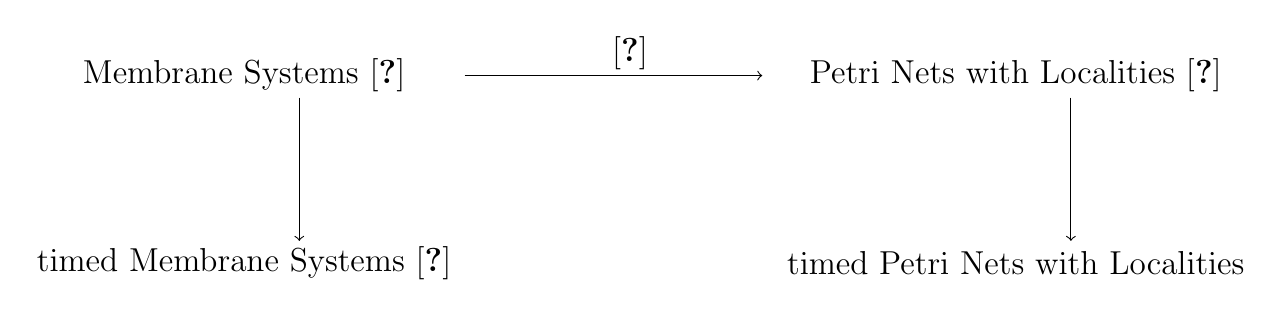
\begin{tikzpicture}[scale=1.4]
\node at (0.0,0.0) {\large Membrane Systems \cite{Paun02}};

\node at (7.0,0.0) {\large Petri Nets with Localities \cite{Kleijn06}};

\draw[->] (2.0,0.0) -- (4.7,0.0);

\node at (3.5,0.2) {\large \cite{Kleijn06}};

\draw[->] (0.5,-0.2) -- (0.5,-1.5);

\draw[->] (7.5,-0.2) -- (7.5,-1.5);

\node at (0.0,-1.7) {\large timed Membrane Systems
\cite{Cavaliere05}};

\node at (7.0,-1.7) {\large timed Petri Nets with Localities};

\end{tikzpicture}
\end{center}

\medskip

\noindent Surprisingly, we prove that adding timing aspects does
not lead to more powerful formalisms, and the new links are expressed
by the following diagram.

\medskip

\begin{center}
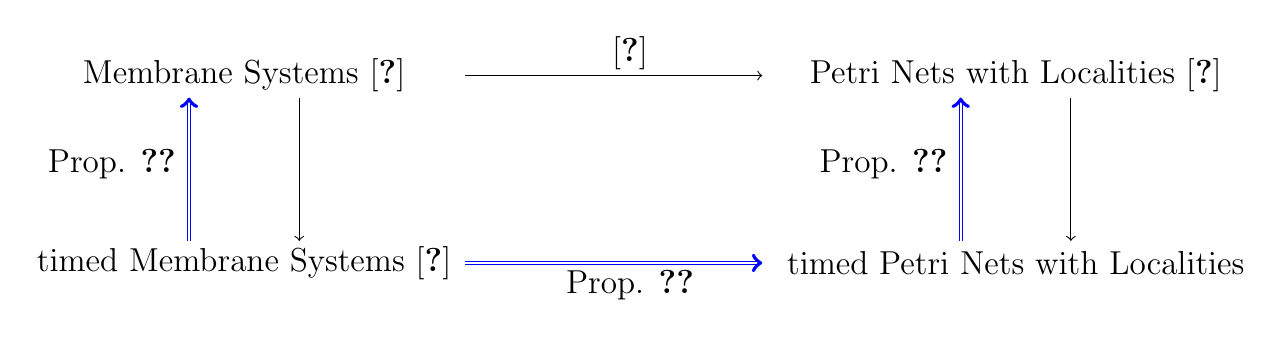
\begin{tikzpicture}[scale=1.4]
\node at (0.0,0.0) {\large Membrane Systems \cite{Paun02}};

\node at (7.0,0.0) {\large Petri Nets with Localities \cite{Kleijn06}};

\draw[->] (2.0,0.0) -- (4.7,0.0);

\node at (3.5,0.2) {\large \cite{Kleijn06}};

\draw[->] (0.5,-0.2) -- (0.5,-1.5);

\draw[<-,double,blue] (-0.5,-0.2) -- (-0.5,-1.5);

\node at (-1.2,-0.8) {\large Prop. \ref{tPtoP}};

\draw[->] (7.5,-0.2) -- (7.5,-1.5);

\draw[<-,double,blue] (6.5,-0.2) -- (6.5,-1.5);

\node at (5.8,-0.8) {\large Prop. \ref{tPNtoPN}};

\node at (0.0,-1.7) {\large timed Membrane Systems
\cite{Cavaliere05}};

\node at (7.0,-1.7) {\large timed Petri Nets with Localities};

\draw[->,double,blue] (2.0,-1.7) -- (4.7,-1.7);

\node at (3.5,-1.9) {\large Prop. \ref{proposition:corresp}};

\end{tikzpicture}
\end{center}

\medskip

We prove that timing does not increase the expressive power of both membrane
systems and Petri nets with localities. However the timed formalisms are able
to describe more naturally some real systems involving timing. Although there
are few extensions with time for both membrane systems and Petri nets, it does
not exist a connection between these timed extensions. An attempt is presented
in \cite{Profir05} by using a software simulation (and having some decidability
aims). We relate timed membrane systems to timed Petri nets with localities
following the research line of \cite{Kleijn06}, and prove an operational
correspondence between them.

\section{Timed Membrane Systems}
\label{section:timed_symanti}

Membrane systems (also called P systems) are introduced by P\u aun as a
model of distributed, parallel and nondeterministic systems inspired by
cell biology \cite{Paun02}. A cell is divided in various compartments, each
compartment with a different task, with all of them working simultaneously
to accomplish a more general task for the whole system. The membranes
determine regions where objects and evolution rules can be placed. The
objects evolve according to the rules associated with each region, and the
regions cooperate in order to maintain the proper behaviour of the whole
system. The application of evolution rules is done in parallel, and is
eventually regulated by priority relationships between rules. Several
results and variants of membrane systems (inspired by different aspects of
living cells like symport and antiport communication through membranes,
catalytic objects, membrane charge, etc.) are presented in~\cite{Paun02}.
Various applications of membrane systems are presented in \cite{Ciobanu06}.
Links between membrane systems and process calculi are presented in
\cite{Ciobanu10}. An updated bibliography can be found on the membrane
systems webpage {\sf http://ppage.psystems.eu}.

The structure of a membrane system is represented by a tree (with the skin as
its root), or equivalently, by a string of correctly matching parentheses where
each pair of matching parentheses corresponds to a membrane. Graphically, a
membrane structure is represented by a Venn diagram in which two sets can be
either disjoint, or one is the subset of the other. A membrane without any other
membrane inside is said to be elementary. The membranes are labelled in a
one-to-one manner.

Let  be the set of positive integers, and  a finite alphabet of
symbols. A multiset over  is a mapping . We use the
string representation of multisets that is widely accepted and used in membrane
systems; a multiset  described by  means that  appears twice in
, while  appears five times in . We use a global clock to simulate the
passage of time. The following definition of timed membrane systems is similar
to that introduced in \cite{Cavaliere05}, but without considering catalysts,
signal-promoters and output region.

\begin{definition}
\label{definition:timed_symanti} A {\rm timed membrane system}
 is defined by
\begin{itemize}
\item[]  is an alphabet (its elements are called
{\rm objects});

\item[]  describes the {\rm membrane
structure}, namely a structure consisting of a hierarchy of 
membranes labelled from  to  which are either disjoint or
included; we distinguish the external membrane, usually called
``skin'';

\item[]  are finite multisets over ; 
represents the multiset of objects associated to membrane ;  is the initial degree of the system;

\item[]  are finite sets of
evolution rules over  associated with the membranes of ; the
rules are of the form , where  and  is
a multiset from ;

\item  is a
(computable) function indicating the execution time of each
evolution rule; the time evolves according to a global clock that
starts from 0 and splits time in equal intervals (units of time).
\end{itemize}
\end{definition}

The membrane structure and the multisets in  determine a
configuration of the system. We can pass from a configuration to
another one by using the evolution rules. The use of a rule
 in a region with a multiset  means to subtract
the multiset identified by  from , and then add the multiset
represented by~.
Since the right hand side  of a rule consists only of messages,
an object introduced by a rule cannot evolve in the same step by
means of another rule. If a message appears in  in the form
, then it remains in the same region. If it appears as
, then a copy of  is introduced in the child membrane
with the label ; if a child membrane with the label  does not
exist, then the rule cannot be applied. If it appears as ,
then a copy of the object  is introduced in the parent (surrounding)
membrane. The system may contain rules which are never applicable,
and also rules which send objects out of the skin.

The evolution rules in a membrane are applied in a
maximal parallel manner, and all membranes evolves in parallel. At
each tick of the (global) clock, all the rules that can be applied
must be applied in a maximal parallel manner (this means that no
further rule could be applied at the same time unit). An evolution
rule  started at the -th tick of the clock ends its execution
at the -th tick, meaning that the newly created objects by
rule  can be used starting from the -th tick of the
clock. When a rule starts, the objects from the left hand side of
the rule become unavailable for other rules.

\medskip

\begin{figure}[ht]
\begin{tabular}{c@{\hspace{6ex}}c}
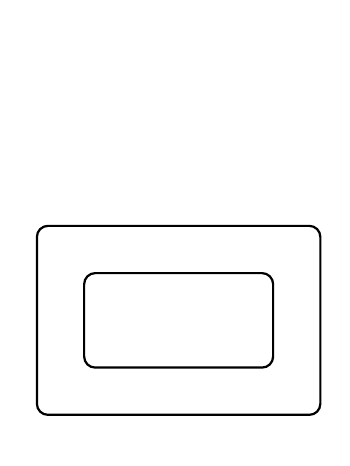
\begin{tikzpicture}[scale=1.2]
\node at (1.0,3.0) {};

\node at (1.0,2.5) {};

\node at (1.0,4.0) {};

\node at (1.0,3.5) {};

\draw[thick,rounded corners=4pt] (0.0,0.5) rectangle (2.0,1.5);

\node at (0.0,0.35) {};

\node at (1.0,1.0) {};

\draw[thick,rounded corners=4pt] (-0.5,0.0) rectangle (2.5,2.0);

\node at (-0.5,-0.15) {};

\node at (1.0,0.25) {};
\end{tikzpicture}&
\begin{minipage}{7.7cm}\vspace{-33ex}{As an example, we consider
a membrane system with two nested membranes (the inner membrane
labelled by , the outer membrane labelled by ), two sets
 and  of evolution rules having the execution times ,
, , , a global clock and two symbols
( and ). Initially, membrane~ contains the multiset
, and membrane~ contains the multiset .}

\end{minipage}\\
\end{tabular}
\centering\vspace{-3ex}\caption{A Timed Membrane System}
\label{figure:example_membrane}
\end{figure}

In what follows we define the configurations of a membrane system,
and the transition system given by considering each of the
transition steps defined by maximally parallel rewriting and
parallel communication, as in \cite{CiobanuHandbook}. Let  be a
finite alphabet of objects over which we consider the free
commutative monoid  whose elements are multisets (the empty
multiset is denoted by ). Objects together with a target indication
are enclosed in messages of form , , and
. For the sake of simplicity, hereinafter we consider
that the messages with the same target indication merge into one
message:

\centerline{,
, ,}

\noindent
with ,  a non-empty
set, and  a family of multisets over .

A configuration for a membrane system is a tuple
, namely the multisets of all regions together
with the value of the global clock. An intermediary configuration is
a tuple in which the objects have associated target indications.
Each membrane system has an initial configuration which is
characterized by the initial multiset of objects for each membrane
of the initial membrane structure of the system.
For two configurations  and  of , we say that there is a
transition from  to , and write , if the
following {\it steps} are executed in the given order:
\begin{enumerate}
\item {\em maximal parallel rewriting step}
():
each membrane evolves in a maximal parallel manner;
\item {\em parallel communication of objects through membranes}
(), by sending and receiving messages.
\end{enumerate}
The last step takes place only if there are messages resulting from
the first step. If the first step is not possible, then neither is
the second step, and we say that the system has reached a {\em halting
configuration}. According to \cite{Andrei07}, a transition step
between two configurations  is given by: 
iff  and  are related by the following relation: .
Starting from a configuration without messages, we apply the ``mpr''
step and get an intermediate configuration; if we have messages,
then we apply the ``tar'' step. If the last configuration has no
messages, then we say that the transition relation  is
well-defined as an evolution step between the first and last
configurations.

The evolution of the system  at time step , from a
configuration  to another configuration
 is made by applying
a multiset of rules  in a maximally parallel manner.
If the multiset  of rules is empty, then
only the clock is incremented (from  to ).
Given a multiset of rules ,
we denote by  the multiset
of objects in the left hand sides of the rules in  which are
associated to membrane . In a similar way, by
 is
denoted the multiset of objects in the right hand sides of the rules
in  applied at time  which is associated to membrane  after
 units of time. We also denote by  the
maximum delay inferred by the rules of~.  evolves to  by a
multiset  of rules (this is denoted by
) if for each membrane  the
following conditions~hold:
\begin{enumerate}
\item[] ;
\item[] there is no rule  such that
;
\item[] for each , .
\end{enumerate}
According to , a configuration  has in each membrane labelled by 
enough objects to enable the execution of the multiset  of rules.
The maximal parallelism is captured by , saying that an extra
evolution rule cannot be added to . Condition  describes
the effect of the rules application by adding all the objects having
 created in the last  steps which are ready to be
used in the membrane system evolution. Before incrementing the
global clock, all multisets  are transformed into
 for .

\begin{proposition}\label{tPtoP}
For every timed membrane system  there exists an untimed membrane system
 that
simulates the evolution of  (restricted to the elements of
). Formally, for all  and  we have
, where  and  are the multisets of
objects from membrane  of  and  at step~.
\end{proposition}

\begin{proof} In what follows we show how starting from
a timed membrane system 
 we may construct an untimed membrane system
, where
\begin{itemize}
\item , where ;
\item  and  for ;
\item for each rule  of ,  having , we add  to ;
\item for each rule  of ,  having , we add to  the following sets of rules
which simulate properly the passage of  units of time:
\begin{itemize}
\item , where  is derived from  by
replacing each  by ;
\item , ;
\item .
\end{itemize}
\end{itemize}
We show that each step of the timed membrane system can be simulated
by the corresponding untimed membrane system, using induction
on the number of steps (time units) in timed membrane system.

Firstly, we consider a configuration
 of the timed membrane system and a
maximal multiset  of rules such that
. The resulting configuration
 is given by
 for all  and . Following the construction above, the
initial configuration of the untimed membrane system is
 where  for
all  and .  is the multiset of rules
obtained from  such that
. The resulting
configuration  is given by
 for all  and . This configuration contains all the elements of
 and some additional objects from  introduced to simulate
properly the passage of time. Regarding the elements , it
results that , namely
. Therefore  equals  regarding
the elements of  (we ignore the new elements of 
because they are used only to simulate the passage of time).

Secondly, we consider a configuration
 of the timed membrane system and a
maximal multiset  of rules such that
. The resulting
configuration   is
given by
 for all  and . In the same
time, the multisets  are transformed into
 for . Following the
construction above, the configuration of the untimed membrane system
is , where 
for all , and  for all . This means that
for all , the multiset  contains all the
objects from  and some additional objects from . For
each  from the multiset , the multiset 
contains additional objects . The restriction  used when creating the object  in membrane  means
that an object  has appeared in the right hand side of a rule
from timed membrane systems in the last  units of time,
but has to wait  units of time until it should be added to
membrane  in timed membrane systems.  is the multiset of
rules obtained from  such that
, with
 for all  and . Moreover, in this step some objects of  are
transformed into objects of  by applying the generic rule  (the other objects  are transformed into
objects  by applying the generic rules ). Finally, the number of objects 
obtained in  at this step corresponds to
. It results that
, namely
. Therefore  equals
 regarding the elements of  (we ignore the
elements  because they are used only to simulate the passage of time).
\end{proof}

In what follows we give an example that illustrates the statement of
Proposition \ref{tPtoP}.

\begin{example}
We consider a timed membrane system ,
where:
\begin{itemize}
\item ; \qquad ; \qquad
; \qquad ;
\item ; \qquad
; \qquad
 , .
\end{itemize}

\noindent Since the initial configuration of the timed membrane
system  is , then the evolution of the timed
membrane system in terms of configurations is:

  
 
  

\noindent Graphically this can be depicted as:

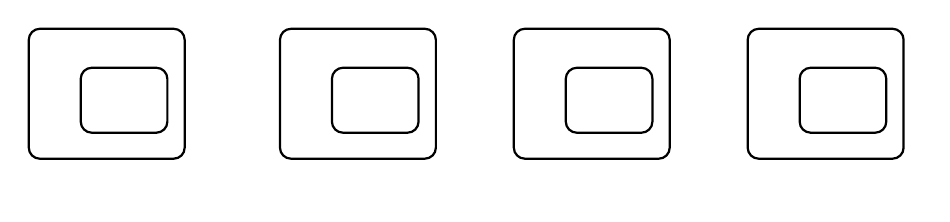
\begin{tikzpicture}[scale=1.1]
\begin{scope}[xshift=-0.2cm]
\draw[thick,rounded corners=4pt] (1.0,0.5) rectangle (2.8,2.0);

\node at (2.9,0.6) {};

\node at (1.3,1.25) {};

\node at (3.35,1.25) {};

\begin{scope}[xshift=1.6cm,yshift=-0.2cm]
\draw[thick,rounded corners=4pt] (0.0,1.0) rectangle (1.0,1.75);

\node at (1.1,1.0) {};

\node at (0.5,1.35) {};
\end{scope}

\node at (2,0.2) {};
\end{scope}

\begin{scope}[xshift=2.7cm]
\draw[thick,rounded corners=4pt] (1.0,0.5) rectangle (2.8,2.0);

\node at (2.9,0.6) {};

\node at (1.3,1.25) {};

\node at (3.35,1.25) {};

\begin{scope}[xshift=1.6cm,yshift=-0.2cm]
\draw[thick,rounded corners=4pt] (0.0,1.0) rectangle (1.0,1.75);

\node at (1.1,1.0) {};

\node at (0.5,1.35) {};
\end{scope}

\node at (2,0.2) {};
\end{scope}

\begin{scope}[xshift=5.4cm]
\draw[thick,rounded corners=4pt] (1.0,0.5) rectangle (2.8,2.0);

\node at (2.9,0.6) {};

\node at (1.3,1.25) {};

\node at (3.35,1.25) {};

\begin{scope}[xshift=1.6cm,yshift=-0.2cm]
\draw[thick,rounded corners=4pt] (0.0,1.0) rectangle (1.0,1.75);

\node at (1.1,1.0) {};

\node at (0.5,1.35) {};
\end{scope}

\node at (2,0.2) {};
\end{scope}

\begin{scope}[xshift=8.1cm]
\draw[thick,rounded corners=4pt] (1.0,0.5) rectangle (2.8,2.0);

\node at (2.9,0.6) {};

\node at (1.3,1.25) {};

\begin{scope}[xshift=1.6cm,yshift=-0.2cm]
\draw[thick,rounded corners=4pt] (0.0,1.0) rectangle (1.0,1.75);

\node at (1.1,1.0) {};

\node at (0.5,1.35) {};
\end{scope}

\node at (2,0.2) {};
\end{scope}
\end{tikzpicture}

\noindent We construct an untimed membrane system
, where:
\begin{itemize}
\item ; \qquad ; \qquad
; \qquad ;
\item ; \qquad
.
\end{itemize}

\noindent Since the initial configuration of the untimed membrane
system  is the same as the initial configuration of the timed
membrane system , namely , then the evolution of
the untimed membrane system in terms of configurations is:

 
  
  

\noindent Graphically this can be depicted as:

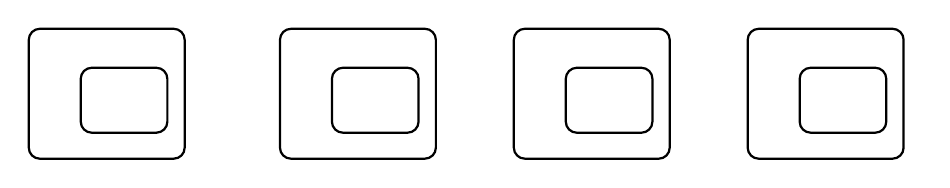
\begin{tikzpicture}[scale=1.1]
\begin{scope}[xshift=-0.2cm]
\draw[thick,rounded corners=4pt] (1.0,0.5) rectangle (2.8,2.0);

\node at (2.9,0.6) {};

\node at (1.3,1.25) {};

\node at (3.35,1.25) {};

\begin{scope}[xshift=1.6cm,yshift=-0.2cm]
\draw[thick,rounded corners=4pt] (0.0,1.0) rectangle (1.0,1.75);

\node at (1.1,1.0) {};

\node at (0.5,1.35) {};
\end{scope}

\end{scope}

\begin{scope}[xshift=2.7cm]
\draw[thick,rounded corners=4pt] (1.0,0.5) rectangle (2.8,2.0);

\node at (2.9,0.6) {};

\node at (1.3,1.25) {};

\node at (3.35,1.25) {};

\begin{scope}[xshift=1.6cm,yshift=-0.2cm]
\draw[thick,rounded corners=4pt] (0.0,1.0) rectangle (1.0,1.75);

\node at (1.1,1.0) {};

\node at (0.5,1.35) {};
\end{scope}

\end{scope}

\begin{scope}[xshift=5.4cm]
\draw[thick,rounded corners=4pt] (1.0,0.5) rectangle (2.8,2.0);

\node at (2.9,0.6) {};

\node at (1.3,1.25) {};

\node at (3.35,1.25) {};

\begin{scope}[xshift=1.6cm,yshift=-0.2cm]
\draw[thick,rounded corners=4pt] (0.0,1.0) rectangle (1.0,1.75);

\node at (1.1,1.0) {};

\node at (0.5,1.35) {};
\end{scope}

\end{scope}

\begin{scope}[xshift=8.1cm]
\draw[thick,rounded corners=4pt] (1.0,0.5) rectangle (2.8,2.0);

\node at (2.9,0.6) {};

\node at (1.3,1.25) {};

\begin{scope}[xshift=1.6cm,yshift=-0.2cm]
\draw[thick,rounded corners=4pt] (0.0,1.0) rectangle (1.0,1.75);

\node at (1.1,1.0) {};

\node at (0.5,1.35) {};
\end{scope}

\end{scope}
\end{tikzpicture}

\noindent If we are interested only in the symbols of 
in the untimed evolution, then we have:

\begin{tabular}{c@{\hspace{0ex}}c@{\hspace{0ex}}c@{\hspace{0ex}}c
@{\hspace{0ex}}c@{\hspace{0ex}}c@{\hspace{0ex}}c@{\hspace{0ex}}c
@{\hspace{0ex}}c@{\hspace{0ex}}c @{\hspace{0ex}}c
@{\hspace{0ex}}c@{\hspace{0ex}}c@{\hspace{0ex}}c@{\hspace{0ex}}c}

,&,& &&
,&,& &
&,&,&&
 & ,&,&\\

 &&&&  &&&&  & &&& &\\

,& &&
& ,&& &&
,&&
&&
,&&\\
\end{tabular}

\noindent and thus the statement of Proposition \ref{tPtoP} holds.

\end{example}

It is easy to prove that the class of timed membrane systems
includes the class of untimed membrane systems, since we can assign
 to all the rules by the timing function .

\section{Timed Petri Nets with Localities}
\label{subsection:cpn}

An extension of Petri nets with localities is defined by adding
delays to transitions (like in coloured Petri nets \cite{Jensen92}).
The value of the global clock is kept in a variable .

\begin{definition} A timed Petri net with localities
 is given~by:
\begin{enumerate}
\item[] finite disjoint sets  of places and  of
transitions;
\item[] a weight function ;
\item[] a locality mapping ;
\item[] a delay mapping ;
\item[] an initial marking .
\end{enumerate}
\end{definition}
\noindent If  for some , then  is an arc from the place (transition) 
to the transition (place) . The locality mapping  defines sets
of transitions called localities (depending on the number associated
to each transition). The delay mapping  introduces a time delay to
each object created by a transition; the delays indicate how long
the objects cannot be used in other transitions. The initial marking
 assigns to each place a number of tokens, and value  to the
global clock .

\begin{figure}[ht]
\begin{tabular}{c@{\hspace{4ex}}c}
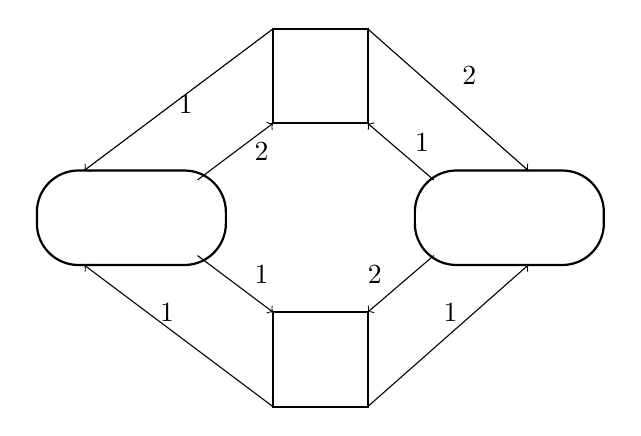
\begin{tikzpicture}[scale=1.2]
\begin{scope}[xshift=4cm,yshift=1cm]
\draw[thick,rounded corners=15pt] (0.0,0.5) rectangle (2.0,1.5);

\node at (0.0,0.5) {};

\node at (1.0,1.0) {};
\end{scope}

\begin{scope}[xshift=8cm,yshift=1cm]
\draw[thick,rounded corners=15pt] (0.0,0.5) rectangle (2.0,1.5);

\node at (2.0,0.5) {};

\node at (1.0,1.0) {};
\end{scope}


\begin{scope}[xshift=6.5cm,yshift=-0.5cm]
\draw[thick,rounded corners=0pt] (0.0,0.5) rectangle (1.0,1.5);

\node at (0.5,1.0) {};
\end{scope}

\begin{scope}[xshift=6.5cm,yshift=2.5cm]
\draw[thick,rounded corners=0pt] (0.0,0.5) rectangle (1.0,1.5);

\node at (0.5,1.0) {};
\end{scope}

\draw[->] (5.7,1.6) -- (6.5,1.0);

\node at (6.2,1.4)[anchor=west] { 1};

\draw[->] (6.5,0.0) -- (4.5,1.5);

\node at (5.2,1.0)[anchor=west] { 1};

\draw[->] (8.2,1.6) -- (7.5,1.0);

\node at (7.4,1.4)[anchor=west] { 2};

\draw[->] (7.5,0.0) -- (9.2,1.5);

\node at (8.2,1.0)[anchor=west] { 1};

\draw[->] (5.7,2.4) -- (6.5,3.0);

\node at (6.2,2.7)[anchor=west] { 2};

\draw[->] (6.5,4.0) -- (4.5,2.5);

\node at (5.4,3.2)[anchor=west] { 1};

\draw[->] (8.2,2.4) -- (7.5,3.0);

\node at (7.9,2.8)[anchor=west] { 1};

\draw[->] (7.5,4.0) -- (9.2,2.5);

\node at (8.4,3.5)[anchor=west] { 2};
\end{tikzpicture}&
\begin{minipage}{7cm}\vspace{-28ex} { Places are drawn as
rounded lines with tokens placed inside. A transition is drawn as a
rectangle containing a label, and the delay it introduces for the
newly created tokens. Transitions are connected to places by
weighted directed arcs.}
\end{minipage}\\
\end{tabular}
\centering\vspace{-2ex}\caption{A Timed Petri Net}
\label{figure:example_petri}
\end{figure}

Markings represent global states of the timed
Petri nets with localities, and they are defined as functions from  to . A Petri net  evolves at a
time step  from a marking~ to another marking~ by a
multiset of transitions  (e.g., 
for  means that  contains twice the transition ). If
the multiset  of transitions is empty, then the only action is
incrementing the global clock . Given a multiset of transitions
, we denote by  the
multiset of tokens associated to the input arcs () of all
transitions . In a similar way, by
 is
denoted the multiset of tokens associated to the output arcs
() which are added to their corresponding places after
 units of time ( represents the current time). We denote by
 the maximum delay inferred by the
transitions of . A marking  leads in a max-enabled way to a
marking  via a multiset  of transitions (denoted by
) if  and for each place  the following conditions hold:
\begin{itemize}
\item[] ;
\item[] there is {\bf no} transition  such that
;
\item[] .
\end{itemize}
According to , a marking  has in each place  enough
tokens to enable the execution of the multiset  of transitions.
The maximal parallelism is captured by , saying that an extra
transition cannot be added to . Condition  describes the
effect of the transitions application by adding all the tokens
having  created in the last  steps which are ready
to be used in Petri nets evolution. Before incrementing the global
clock, all the multisets  are transformed into
 for .

\begin{proposition}
\label{tPNtoPN} For every timed Petri net with localities
 there exists a Petri net with
localities  that simulates the
evolution of  (with respect to places of ).
Formally, for all  and  we have
, where  and  are markings of  and
 at step~.
\end{proposition}

\begin{proof} In what follows we show how starting from
a timed Petri net with localities 
, we construct an untimed Petri net with localities
, where
\begin{itemize}
\item for every  and  such that , we
consider additional places 
in ; if  then only ;

\item for every  and  such that , we consider
additional transitions   in ; if
 then ;

\item for every  and  such that ,
we consider the weights  in :
\begin{itemize}
\item if  then ;
\item if  then , and \\

for ;
\end{itemize}

\item for every  and  such that
, we consider the following weights  in
:
if  then , else ;

\item for every , we take the same locality label
 for the new transitions ;

\item if  then
, and if  then  .
\end{itemize}
We show that each step of the timed Petri nets with localities can
be simulated by the corresponding untimed Petri nets with localities;
we prove this by induction on the number of steps (time units)
in timed Petri nets with localities.

Firstly, we consider a marking  of the timed Petri net with
localities and a multiset of transitions  such that . The resulting marking  is given by
 for all . Following
the construction above, the initial marking of the untimed Petri net
with localities is , where  for all .
 is the multiset of transitions obtained from  such that
. The resulting marking  is
given by  for all , where .
This marking contains all the places of  and some additional
places from . Regarding the places , it results that
, namely . Therefore
 equals  regarding the number of tokens from the places
of  (we ignore the new places of  because they do not play
any role at this step).

Secondly, we consider a marking  of the timed Petri net with localities
and a multiset  of transitions such that . The
resulting configuration  is given by  for all . In the same time, the
multisets of tokens  are renamed by  for all
 and . Following the construction above,
the marking of the untimed Petri net with localities is , where
 for all , and  for all additional , 
and . This means that the common places of both nets have
the same number of tokens, while for the additional places appearing only in
 we add tokens such that for each token from  obtained
after firing the transition , the place  contains a token. The
restriction  (used when creating a token in a new
place  of ) means that a token appears on an output arc of
transition  in timed Petri nets during the last  units of time;
this token has to wait  units of time until it is added to place  of .
The multiset of rules  is obtained from  such that , with  for
all . Moreover, in this step some tokens are transferred from places
of  into places of  by firing the transitions  (the other tokens
from places  are transferred into places 
by firing the transitions ). Thus, the number of tokens obtained in
places  at each step  is equal to . It
results that , namely
 for all . Therefore  equals
 regarding the number of tokens from the places of  (we ignore the
remaining places  because they are used only to simulate the
passage of time).
\end{proof}

\begin{example}
We consider a timed Petri net with localities
, where
\begin{itemize}
\item ; \qquad
;

\item ; \qquad ; \qquad
; \qquad ;

\item 

\item ; \qquad ; \qquad .
\end{itemize}

\noindent Graphically the system at time unit  can be
represented as follows:

\begin{center}
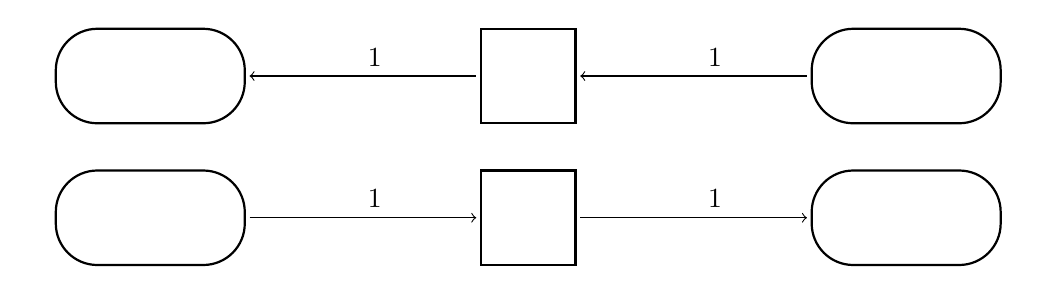
\begin{tikzpicture}[scale=1.2]
\begin{scope}[xshift=0cm,yshift=0cm]
\begin{scope}[xshift=2cm,yshift=0cm]
\draw[thick,rounded corners=15pt] (0.0,0.5) rectangle (2.0,1.5);

\node at (-0.2,0.5) {};

\node at (1.0,1.0) {};
\end{scope}

\begin{scope}[xshift=10cm,yshift=0cm]
\draw[thick,rounded corners=15pt] (0.0,0.5) rectangle (2.0,1.5);

\node at (2.2,0.5) {};

\node at (1.0,1.0) {};
\end{scope}


\begin{scope}[xshift=6.5cm,yshift=0cm]
\draw[thick,rounded corners=0pt] (0.0,0.5) rectangle (1.0,1.5);

\node at (0.5,1.0) {};
\end{scope}

\draw[<-] (4.05,1.0) -- (6.45,1.0);

\node at (5.2,1.2)[anchor=west] { 1};

\draw[<-] (7.55,1.0) -- (9.95,1.0);

\node at (8.8,1.2)[anchor=west] { 1};
\end{scope}



\begin{scope}[xshift=0cm,yshift=-1.5cm]
\begin{scope}[xshift=2cm,yshift=0cm]
\draw[thick,rounded corners=15pt] (0.0,0.5) rectangle (2.0,1.5);

\node at (-0.2,0.5) {};

\node at (1.0,1.0) {};
\end{scope}

\begin{scope}[xshift=10cm,yshift=0cm]
\draw[thick,rounded corners=15pt] (0.0,0.5) rectangle (2.0,1.5);

\node at (2.2,0.5) {};

\node at (1.0,1.0) {};
\end{scope}


\begin{scope}[xshift=6.5cm,yshift=0cm]
\draw[thick,rounded corners=0pt] (0.0,0.5) rectangle (1.0,1.5);

\node at (0.5,1.0) {};
\end{scope}

\draw[->] (4.05,1.0) -- (6.45,1.0);

\node at (5.2,1.2)[anchor=west] { 1};

\draw[->] (7.55,1.0) -- (9.95,1.0);

\node at (8.8,1.2)[anchor=west] { 1};
\end{scope}
\end{tikzpicture}
\end{center}

\noindent For  and , the timed Petri net with localities can
be represented as follows:

\begin{center}
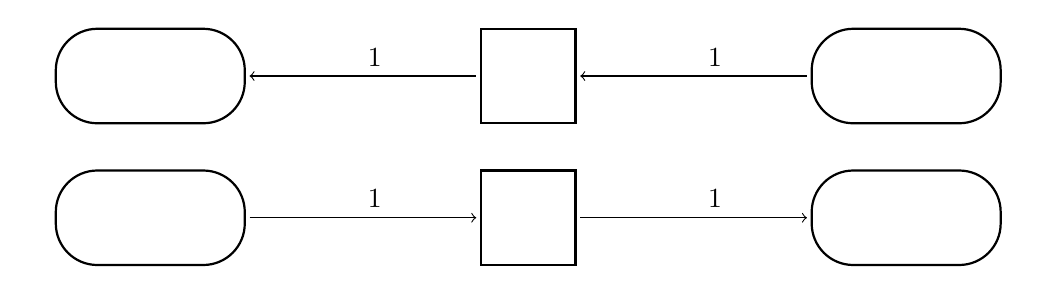
\begin{tikzpicture}[scale=1.2]
\begin{scope}[xshift=0cm,yshift=0.0cm]
\begin{scope}[xshift=2cm,yshift=0cm]
\draw[thick,rounded corners=15pt] (0.0,0.5) rectangle (2.0,1.5);

\node at (-0.2,0.5) {};

\node at (1.0,1.0) {};
\end{scope}

\begin{scope}[xshift=10cm,yshift=0cm]
\draw[thick,rounded corners=15pt] (0.0,0.5) rectangle (2.0,1.5);

\node at (2.2,0.5) {};
\end{scope}


\begin{scope}[xshift=6.5cm,yshift=0cm]
\draw[thick,rounded corners=0pt] (0.0,0.5) rectangle (1.0,1.5);

\node at (0.5,1.0) {};
\end{scope}

\draw[<-] (4.05,1.0) -- (6.45,1.0);

\node at (5.2,1.2)[anchor=west] { 1};

\draw[<-] (7.55,1.0) -- (9.95,1.0);

\node at (8.8,1.2)[anchor=west] { 1};
\end{scope}

\begin{scope}[xshift=0cm,yshift=-1.5cm]
\begin{scope}[xshift=2cm,yshift=0cm]
\draw[thick,rounded corners=15pt] (0.0,0.5) rectangle (2.0,1.5);

\node at (-0.2,0.5) {};

\end{scope}

\begin{scope}[xshift=10cm,yshift=0cm]
\draw[thick,rounded corners=15pt] (0.0,0.5) rectangle (2.0,1.5);

\node at (2.2,0.5) {};

\node at (1.0,1.0) {};
\end{scope}


\begin{scope}[xshift=6.5cm,yshift=0cm]
\draw[thick,rounded corners=0pt] (0.0,0.5) rectangle (1.0,1.5);

\node at (0.5,1.0) {};
\end{scope}

\draw[->] (4.05,1.0) -- (6.45,1.0);

\node at (5.2,1.2)[anchor=west] { 1};

\draw[->] (7.55,1.0) -- (9.95,1.0);

\node at (8.8,1.2)[anchor=west] { 1};
\end{scope}
\end{tikzpicture}
\end{center}


\noindent while for all  we have the following representation

\begin{center}
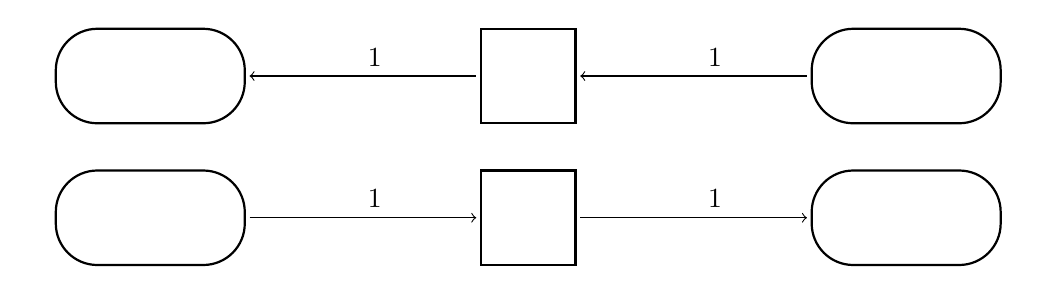
\begin{tikzpicture}[scale=1.2]
\begin{scope}[xshift=0cm,yshift=0.0cm]
\begin{scope}[xshift=2cm,yshift=0cm]
\draw[thick,rounded corners=15pt] (0.0,0.5) rectangle (2.0,1.5);

\node at (-0.2,0.5) {};

\node at (1.0,1.0) {};
\end{scope}

\begin{scope}[xshift=10cm,yshift=0cm]
\draw[thick,rounded corners=15pt] (0.0,0.5) rectangle (2.0,1.5);

\node at (2.2,0.5) {};

\end{scope}


\begin{scope}[xshift=6.5cm,yshift=0cm]
\draw[thick,rounded corners=0pt] (0.0,0.5) rectangle (1.0,1.5);

\node at (0.5,1.0) {};
\end{scope}

\draw[<-] (4.05,1.0) -- (6.45,1.0);

\node at (5.2,1.2)[anchor=west] { 1};

\draw[<-] (7.55,1.0) -- (9.95,1.0);

\node at (8.8,1.2)[anchor=west] { 1};
\end{scope}

\begin{scope}[xshift=0cm,yshift=-1.5cm]
\begin{scope}[xshift=2cm,yshift=0cm]
\draw[thick,rounded corners=15pt] (0.0,0.5) rectangle (2.0,1.5);

\node at (-0.2,0.5) {};

\end{scope}

\begin{scope}[xshift=10cm,yshift=0cm]
\draw[thick,rounded corners=15pt] (0.0,0.5) rectangle (2.0,1.5);

\node at (2.2,0.5) {};

\node at (1.0,1.0) {};
\end{scope}


\begin{scope}[xshift=6.5cm,yshift=0cm]
\draw[thick,rounded corners=0pt] (0.0,0.5) rectangle (1.0,1.5);

\node at (0.5,1.0) {};
\end{scope}

\draw[->] (4.05,1.0) -- (6.45,1.0);

\node at (5.2,1.2)[anchor=west] { 1};

\draw[->] (7.55,1.0) -- (9.95,1.0);

\node at (8.8,1.2)[anchor=west] { 1};
\end{scope}
\end{tikzpicture}
\end{center}


\noindent We construct an untimed Petri net with localities
, where
\begin{itemize}
\item  and
, where  and
;

\item ; \qquad ;

\item 

\item 

\item ; \qquad ; \qquad .
\end{itemize}

\noindent Graphically, the initial system can be represented as follows:

\begin{center}
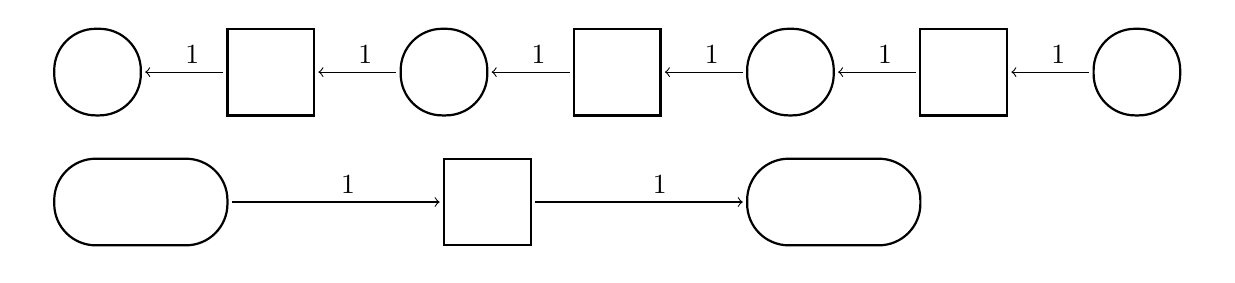
\begin{tikzpicture}[scale=1.1]
\begin{scope}[xshift=0cm,yshift=0cm]
\begin{scope}[xshift=2cm,yshift=0cm]
\draw[thick,rounded corners=15pt] (0.0,0.5) rectangle (1.0,1.5);

\node at (-0.2,0.5) {};

\node at (0.5,1.0) {};
\end{scope}

\begin{scope}[xshift=14cm,yshift=0cm]
\draw[thick,rounded corners=15pt] (0.0,0.5) rectangle (1.0,1.5);

\node at (1.2,0.5) {};

\node at (0.5,1.0) {};
\end{scope}


\begin{scope}[xshift=4cm,yshift=0cm]
\draw[thick,rounded corners=0pt] (0.0,0.5) rectangle (1.0,1.5);

\node at (0.5,1.0) {};
\end{scope}

\begin{scope}[xshift=6cm,yshift=0cm]
\draw[thick,rounded corners=15pt] (0.0,0.5) rectangle (1.0,1.5);

\node at (1.0,0.5) {};

\end{scope}

\begin{scope}[xshift=8cm,yshift=0cm]
\draw[thick,rounded corners=0pt] (0.0,0.5) rectangle (1.0,1.5);

\node at (0.5,1.0) {};
\end{scope}

\begin{scope}[xshift=10cm,yshift=0cm]
\draw[thick,rounded corners=15pt] (0.0,0.5) rectangle (1.0,1.5);

\node at (1.0,0.5) {};
\end{scope}

\begin{scope}[xshift=12cm,yshift=0cm]
\draw[thick,rounded corners=0pt] (0.0,0.5) rectangle (1.0,1.5);

\node at (0.5,1.0) {};
\end{scope}

\draw[<-] (3.05,1.0) -- (3.95,1.0);

\node at (3.4,1.2)[anchor=west] { 1};

\draw[<-] (5.05,1.0) -- (5.95,1.0);

\node at (5.4,1.2)[anchor=west] { 1};

\draw[<-] (7.05,1.0) -- (7.95,1.0);

\node at (7.4,1.2)[anchor=west] { 1};

\draw[<-] (9.05,1.0) -- (9.95,1.0);

\node at (9.4,1.2)[anchor=west] { 1};

\draw[<-] (11.05,1.0) -- (11.95,1.0);

\node at (11.4,1.2)[anchor=west] { 1};

\draw[<-] (13.05,1.0) -- (13.95,1.0);

\node at (13.4,1.2)[anchor=west] {1};
\end{scope}



\begin{scope}[xshift=0cm,yshift=-1.5cm]
\begin{scope}[xshift=2cm,yshift=0cm]
\draw[thick,rounded corners=15pt] (0.0,0.5) rectangle (2.0,1.5);

\node at (-0.2,0.5) {};

\node at (1.0,1.0) {};
\end{scope}

\begin{scope}[xshift=10cm,yshift=0cm]
\draw[thick,rounded corners=15pt] (0.0,0.5) rectangle (2.0,1.5);

\node at (2.2,0.5) {};

\node at (1.0,1.0) {};
\end{scope}


\begin{scope}[xshift=6.5cm,yshift=0cm]
\draw[thick,rounded corners=0pt] (0.0,0.5) rectangle (1.0,1.5);

\node at (0.5,1.0) {};
\end{scope}

\draw[->] (4.05,1.0) -- (6.45,1.0);

\node at (5.2,1.2)[anchor=west] { 1};

\draw[->] (7.55,1.0) -- (9.95,1.0);

\node at (8.8,1.2)[anchor=west] { 1};
\end{scope}
\end{tikzpicture}
\end{center}

\noindent
After one step, we obtain

\begin{center}
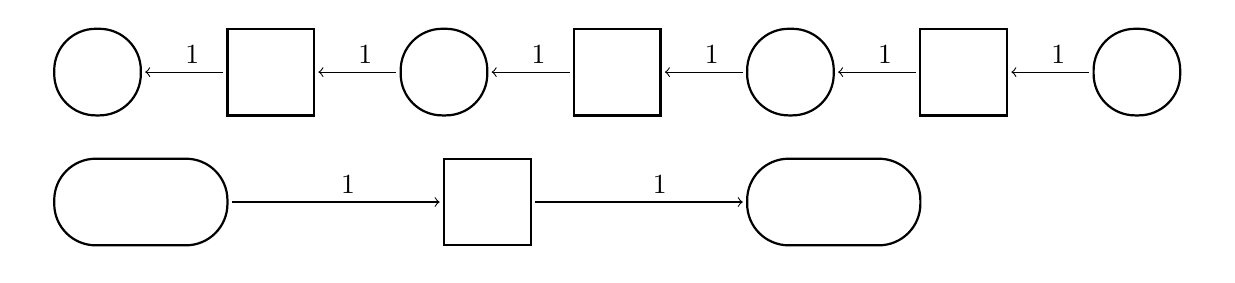
\begin{tikzpicture}[scale=1.1]
\begin{scope}[xshift=0cm,yshift=0cm]
\begin{scope}[xshift=2cm,yshift=0cm]
\draw[thick,rounded corners=15pt] (0.0,0.5) rectangle (1.0,1.5);

\node at (-0.2,0.5) {};

\node at (0.5,1.0) {};
\end{scope}

\begin{scope}[xshift=14cm,yshift=0cm]
\draw[thick,rounded corners=15pt] (0.0,0.5) rectangle (1.0,1.5);

\node at (1.2,0.5) {};

\end{scope}


\begin{scope}[xshift=4cm,yshift=0cm]
\draw[thick,rounded corners=0pt] (0.0,0.5) rectangle (1.0,1.5);

\node at (0.5,1.0) {};
\end{scope}

\begin{scope}[xshift=6cm,yshift=0cm]
\draw[thick,rounded corners=15pt] (0.0,0.5) rectangle (1.0,1.5);

\node at (1.0,0.5) {};

\end{scope}

\begin{scope}[xshift=8cm,yshift=0cm]
\draw[thick,rounded corners=0pt] (0.0,0.5) rectangle (1.0,1.5);

\node at (0.5,1.0) {};
\end{scope}

\begin{scope}[xshift=10cm,yshift=0cm]
\draw[thick,rounded corners=15pt] (0.0,0.5) rectangle (1.0,1.5);

\node at (1.0,0.5) {};

\node at (0.5,1.0) {};
\end{scope}

\begin{scope}[xshift=12cm,yshift=0cm]
\draw[thick,rounded corners=0pt] (0.0,0.5) rectangle (1.0,1.5);

\node at (0.5,1.0) {};
\end{scope}

\draw[<-] (3.05,1.0) -- (3.95,1.0);

\node at (3.4,1.2)[anchor=west] { 1};

\draw[<-] (5.05,1.0) -- (5.95,1.0);

\node at (5.4,1.2)[anchor=west] { 1};

\draw[<-] (7.05,1.0) -- (7.95,1.0);

\node at (7.4,1.2)[anchor=west] { 1};

\draw[<-] (9.05,1.0) -- (9.95,1.0);

\node at (9.4,1.2)[anchor=west] { 1};

\draw[<-] (11.05,1.0) -- (11.95,1.0);

\node at (11.4,1.2)[anchor=west] { 1};

\draw[<-] (13.05,1.0) -- (13.95,1.0);

\node at (13.4,1.2)[anchor=west] { 1};
\end{scope}



\begin{scope}[xshift=0cm,yshift=-1.5cm]
\begin{scope}[xshift=2cm,yshift=0cm]
\draw[thick,rounded corners=15pt] (0.0,0.5) rectangle (2.0,1.5);

\node at (-0.2,0.5) {};
\end{scope}

\begin{scope}[xshift=10cm,yshift=0cm]
\draw[thick,rounded corners=15pt] (0.0,0.5) rectangle (2.0,1.5);

\node at (2.2,0.5) {};

\node at (1.0,1.0) {};
\end{scope}


\begin{scope}[xshift=6.5cm,yshift=0cm]
\draw[thick,rounded corners=0pt] (0.0,0.5) rectangle (1.0,1.5);

\node at (0.5,1.0) {};
\end{scope}

\draw[->] (4.05,1.0) -- (6.45,1.0);

\node at (5.2,1.2)[anchor=west] { 1};

\draw[->] (7.55,1.0) -- (9.95,1.0);

\node at (8.8,1.2)[anchor=west] { 1};
\end{scope}
\end{tikzpicture}
\end{center}

\noindent The system evolves to

\begin{center}
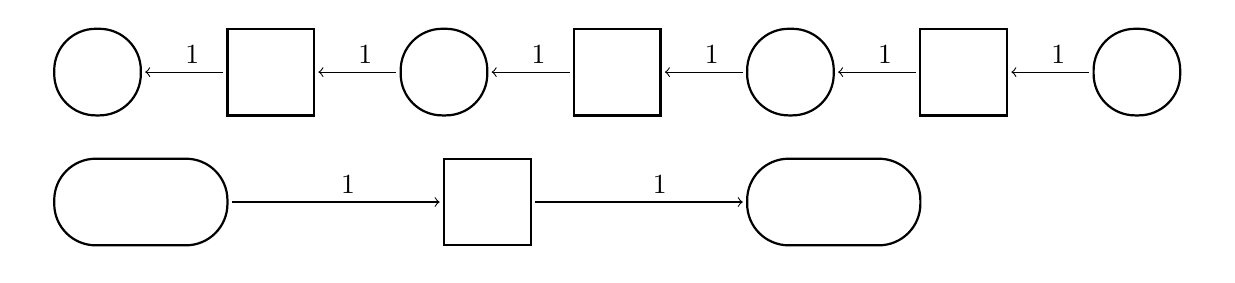
\begin{tikzpicture}[scale=1.1]
\begin{scope}[xshift=0cm,yshift=0cm]
\begin{scope}[xshift=2cm,yshift=0cm]
\draw[thick,rounded corners=15pt] (0.0,0.5) rectangle (1.0,1.5);

\node at (-0.2,0.5) {};

\node at (0.5,1.0) {};
\end{scope}

\begin{scope}[xshift=14cm,yshift=0cm]
\draw[thick,rounded corners=15pt] (0.0,0.5) rectangle (1.0,1.5);

\node at (1.2,0.5) {};

\end{scope}


\begin{scope}[xshift=4cm,yshift=0cm]
\draw[thick,rounded corners=0pt] (0.0,0.5) rectangle (1.0,1.5);

\node at (0.5,1.0) {};
\end{scope}

\begin{scope}[xshift=6cm,yshift=0cm]
\draw[thick,rounded corners=15pt] (0.0,0.5) rectangle (1.0,1.5);

\node at (1.0,0.5) {};

\node at (0.5,1.0) {};

\end{scope}

\begin{scope}[xshift=8cm,yshift=0cm]
\draw[thick,rounded corners=0pt] (0.0,0.5) rectangle (1.0,1.5);

\node at (0.5,1.0) {};
\end{scope}

\begin{scope}[xshift=10cm,yshift=0cm]
\draw[thick,rounded corners=15pt] (0.0,0.5) rectangle (1.0,1.5);

\node at (1.0,0.5) {};


\end{scope}

\begin{scope}[xshift=12cm,yshift=0cm]
\draw[thick,rounded corners=0pt] (0.0,0.5) rectangle (1.0,1.5);

\node at (0.5,1.0) {};
\end{scope}

\draw[<-] (3.05,1.0) -- (3.95,1.0);

\node at (3.4,1.2)[anchor=west] { 1};

\draw[<-] (5.05,1.0) -- (5.95,1.0);

\node at (5.4,1.2)[anchor=west] { 1};

\draw[<-] (7.05,1.0) -- (7.95,1.0);

\node at (7.4,1.2)[anchor=west] { 1};

\draw[<-] (9.05,1.0) -- (9.95,1.0);

\node at (9.4,1.2)[anchor=west] { 1};

\draw[<-] (11.05,1.0) -- (11.95,1.0);

\node at (11.4,1.2)[anchor=west] { 1};

\draw[<-] (13.05,1.0) -- (13.95,1.0);

\node at (13.4,1.2)[anchor=west] { 1};
\end{scope}



\begin{scope}[xshift=0cm,yshift=-1.5cm]
\begin{scope}[xshift=2cm,yshift=0cm]
\draw[thick,rounded corners=15pt] (0.0,0.5) rectangle (2.0,1.5);

\node at (-0.2,0.5) {};
\end{scope}

\begin{scope}[xshift=10cm,yshift=0cm]
\draw[thick,rounded corners=15pt] (0.0,0.5) rectangle (2.0,1.5);

\node at (2.2,0.5) {};

\node at (1.0,1.0) {};
\end{scope}


\begin{scope}[xshift=6.5cm,yshift=0cm]
\draw[thick,rounded corners=0pt] (0.0,0.5) rectangle (1.0,1.5);

\node at (0.5,1.0) {};
\end{scope}

\draw[->] (4.05,1.0) -- (6.45,1.0);

\node at (5.2,1.2)[anchor=west] { 1};

\draw[->] (7.55,1.0) -- (9.95,1.0);

\node at (8.8,1.2)[anchor=west] { 1};
\end{scope}
\end{tikzpicture}
\end{center}

\noindent
The system stops its evolution after reaching the configuration

\begin{center}
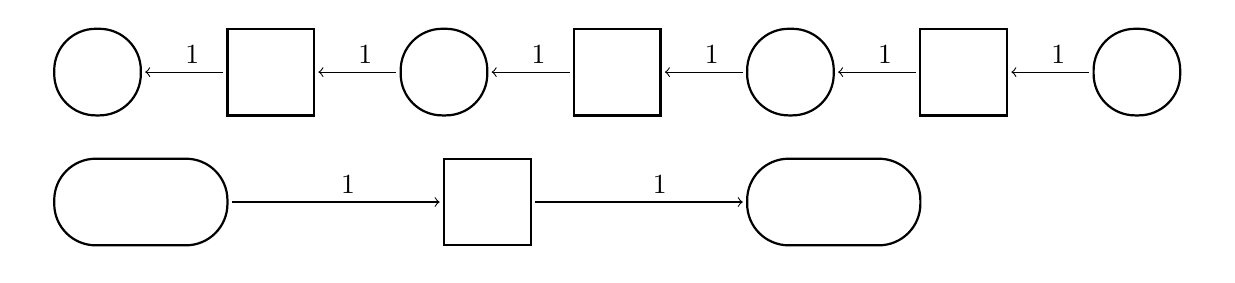
\begin{tikzpicture}[scale=1.1]
\begin{scope}[xshift=0cm,yshift=0cm]
\begin{scope}[xshift=2cm,yshift=0cm]
\draw[thick,rounded corners=15pt] (0.0,0.5) rectangle (1.0,1.5);

\node at (-0.2,0.5) {};

\node at (0.5,1.0) {};
\end{scope}

\begin{scope}[xshift=14cm,yshift=0cm]
\draw[thick,rounded corners=15pt] (0.0,0.5) rectangle (1.0,1.5);

\node at (1.2,0.5) {};

\end{scope}


\begin{scope}[xshift=4cm,yshift=0cm]
\draw[thick,rounded corners=0pt] (0.0,0.5) rectangle (1.0,1.5);

\node at (0.5,1.0) {};
\end{scope}

\begin{scope}[xshift=6cm,yshift=0cm]
\draw[thick,rounded corners=15pt] (0.0,0.5) rectangle (1.0,1.5);

\node at (1.0,0.5) {};

\end{scope}

\begin{scope}[xshift=8cm,yshift=0cm]
\draw[thick,rounded corners=0pt] (0.0,0.5) rectangle (1.0,1.5);

\node at (0.5,1.0) {};
\end{scope}

\begin{scope}[xshift=10cm,yshift=0cm]
\draw[thick,rounded corners=15pt] (0.0,0.5) rectangle (1.0,1.5);

\node at (1.0,0.5) {};


\end{scope}

\begin{scope}[xshift=12cm,yshift=0cm]
\draw[thick,rounded corners=0pt] (0.0,0.5) rectangle (1.0,1.5);

\node at (0.5,1.0) {};
\end{scope}

\draw[<-] (3.05,1.0) -- (3.95,1.0);

\node at (3.4,1.2)[anchor=west] { 1};

\draw[<-] (5.05,1.0) -- (5.95,1.0);

\node at (5.4,1.2)[anchor=west] { 1};

\draw[<-] (7.05,1.0) -- (7.95,1.0);

\node at (7.4,1.2)[anchor=west] { 1};

\draw[<-] (9.05,1.0) -- (9.95,1.0);

\node at (9.4,1.2)[anchor=west] { 1};

\draw[<-] (11.05,1.0) -- (11.95,1.0);

\node at (11.4,1.2)[anchor=west] { 1};

\draw[<-] (13.05,1.0) -- (13.95,1.0);

\node at (13.4,1.2)[anchor=west] { 1};
\end{scope}



\begin{scope}[xshift=0cm,yshift=-1.5cm]
\begin{scope}[xshift=2cm,yshift=0cm]
\draw[thick,rounded corners=15pt] (0.0,0.5) rectangle (2.0,1.5);

\node at (-0.2,0.5) {};
\end{scope}

\begin{scope}[xshift=10cm,yshift=0cm]
\draw[thick,rounded corners=15pt] (0.0,0.5) rectangle (2.0,1.5);

\node at (2.2,0.5) {};

\node at (1.0,1.0) {};
\end{scope}


\begin{scope}[xshift=6.5cm,yshift=0cm]
\draw[thick,rounded corners=0pt] (0.0,0.5) rectangle (1.0,1.5);

\node at (0.5,1.0) {};
\end{scope}

\draw[->] (4.05,1.0) -- (6.45,1.0);

\node at (5.2,1.2)[anchor=west] { 1};

\draw[->] (7.55,1.0) -- (9.95,1.0);

\node at (8.8,1.2)[anchor=west] { 1};
\end{scope}
\end{tikzpicture}
\end{center}

\noindent We notice that indeed, if we refer only to the
markings of the places from  during the evolution of timed and
untimed Petri nets with localities, the markings are the same.

\end{example}

It is easy to prove that the class of timed Petri net with
localities includes the class of Petri net with localities, since we
can assign  to all values of the function~, namely all
transitions fire instantaneously.

\section{Linking Timed Membrane Systems to Timed Petri Nets}
\label{subsection:relationship}

Following the approach given in \cite{Kleijn06} where membrane systems are
translated into Petri nets with localities, we present a translation of timed
membrane systems into timed Petri nets with localities, and then prove an
operational correspondence between them.

\begin{definition}
\label{definition:translation} Let
 be a timed membrane
system. Then the corresponding timed Petri net with localities is
 with its components defined as
follows:

\begin{itemize}
\item  - to each object  of
membrane  there corresponds a place ;

\item  - to
each rule  of membrane  corresponds a transition ;

\item for every place  and every transition 

 and


\item for every place , we have ;
\item for every transition , we have ;
\item for every , we have .
\end{itemize}
\end{definition}

\begin{example}
We consider a timed membrane system ,
where
\begin{itemize}
\item ; \qquad ; \qquad
; \qquad ;
\item ; \qquad
; \qquad
 , .
\end{itemize}

Graphically, the initial configuration can be depicted as:

\begin{center}
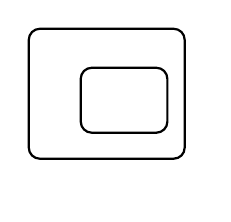
\begin{tikzpicture}[scale=1.1]
\begin{scope}[xshift=-0.2cm]
\draw[thick,rounded corners=4pt] (1.0,0.5) rectangle (2.8,2.0);

\node at (2.9,0.6) {};

\node at (1.3,1.25) {};

\begin{scope}[xshift=1.6cm,yshift=-0.2cm]
\draw[thick,rounded corners=4pt] (0.0,1.0) rectangle (1.0,1.75);

\node at (1.1,1.0) {};

\node at (0.5,1.35) {};
\end{scope}

\node at (2,0.2) {};
\end{scope}

\end{tikzpicture}
\end{center}


\noindent The corresponding timed Petri net with localities is
, where:
\begin{itemize}
\item ; \qquad
;

\item ; \qquad ; \qquad
; \qquad ;

\item 

\item ; \qquad ; \qquad .
\end{itemize}

\noindent Graphically, the system at time unit  can be
represented as

\begin{center}
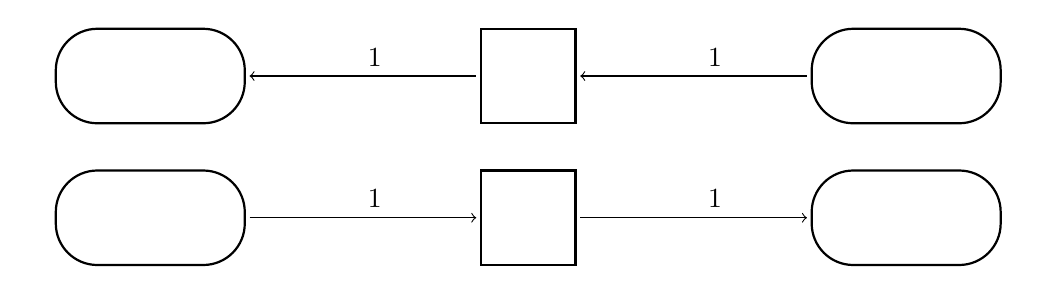
\begin{tikzpicture}[scale=1.2]
\begin{scope}[xshift=0cm,yshift=0cm]
\begin{scope}[xshift=2cm,yshift=0cm]
\draw[thick,rounded corners=15pt] (0.0,0.5) rectangle (2.0,1.5);

\node at (-0.2,0.5) {};

\node at (1.0,1.0) {};
\end{scope}

\begin{scope}[xshift=10cm,yshift=0cm]
\draw[thick,rounded corners=15pt] (0.0,0.5) rectangle (2.0,1.5);

\node at (2.2,0.5) {};

\node at (1.0,1.0) {};
\end{scope}


\begin{scope}[xshift=6.5cm,yshift=0cm]
\draw[thick,rounded corners=0pt] (0.0,0.5) rectangle (1.0,1.5);

\node at (0.5,1.0) {};
\end{scope}

\draw[<-] (4.05,1.0) -- (6.45,1.0);

\node at (5.2,1.2)[anchor=west] { 1};

\draw[<-] (7.55,1.0) -- (9.95,1.0);

\node at (8.8,1.2)[anchor=west] { 1};
\end{scope}



\begin{scope}[xshift=0cm,yshift=-1.5cm]
\begin{scope}[xshift=2cm,yshift=0cm]
\draw[thick,rounded corners=15pt] (0.0,0.5) rectangle (2.0,1.5);

\node at (-0.2,0.5) {};

\node at (1.0,1.0) {};
\end{scope}

\begin{scope}[xshift=10cm,yshift=0cm]
\draw[thick,rounded corners=15pt] (0.0,0.5) rectangle (2.0,1.5);

\node at (2.2,0.5) {};

\node at (1.0,1.0) {};
\end{scope}


\begin{scope}[xshift=6.5cm,yshift=0cm]
\draw[thick,rounded corners=0pt] (0.0,0.5) rectangle (1.0,1.5);

\node at (0.5,1.0) {};
\end{scope}

\draw[->] (4.05,1.0) -- (6.45,1.0);

\node at (5.2,1.2)[anchor=west] { 1};

\draw[->] (7.55,1.0) -- (9.95,1.0);

\node at (8.8,1.2)[anchor=west] { 1};
\end{scope}
\end{tikzpicture}
\end{center}
\end{example}
According to this translation,  denotes the marking
of  corresponding to a configuration  of the
timed membrane system . Moreover, for each multiset  of
applied rules in a timed membrane system, the corresponding multiset
of transitions in timed Petri nets with localities is denoted by
. Using these notations, we have the following operational correspondence:

\begin{proposition}\label{proposition:corresp}
 if and only if .
\end{proposition}
\begin{proof}[Proof] Let us consider the membrane
configuration  . According to Definition
\ref{definition:translation}, we have  for each place
. This is a consequence of the fact that there is a
correspondence between membranes and places, and between the
multiset inside membranes and the marking of the places.
After applying the multiset  of rules in
, we obtain a configuration  where for each
membrane  and each object  we have
. In
the corresponding timed Petri net with localities, starting from the
marking  and applying the multiset  of transitions, we
obtain a new marking  where for each place  we get
. It
is easy to note that ,  and\\
. Therefore, it results that  and
.
\end{proof}

\section{Conclusion}
\label{section:conclusion}

There exist papers in the field of membrane computing in which the
concept of time is used mainly as timers for objects and
membranes \cite{CompMod09,IJCCC10}, and as execution period for
each rule \cite{Cavaliere05,Cavaliere10}.
The idea of adding time to Petri nets is described in
\cite{Peterson81}: ``addition of timing information might
provide a powerful new feature for Petri nets, but may not be
possible in a manner consistent with the basic philosophy of Petri
nets''. Different ways of incorporating timing information into
Petri nets were proposed by many researchers; specific application
fields represent the inspiration for different proposals of
modelling time. For Petri nets with localities \cite{Kleijn06},
time constrains are added in a way inspired by the coloured Petri nets.

In this paper we prove that adding timing to both membrane
systems and Petri nets with localities does not increase the
expressive power of the corresponding untimed formalisms,
establish a link between these timed formalisms by defining
a relationship between timed formalisms under the assumption of
maximal firing, and prove an operational correspondence between
them. This relationship allows to use the Petri nets
tools to verify certain behavioural properties (reachability,
boundedness, liveness and fairness) of membrane systems.
An attempt to use Petri nets software to simulate timing aspects in membrane
systems is presented in \cite{Profir05}.

As further work, we can mention the use of timed membrane systems to model
some biological systems, while Petri nets tools can be used to analyze and verify
automatically the (timing) behavioural properties of these models.

\medskip

\noindent {\bf Acknowledgements}. The work of Bogdan Aman is
supported by POSDRU/89/1.5/S/49944.



\begin{thebibliography}{1}

\providecommand{\urlalt}[2]{\href{#1}{#2}}
\providecommand{\doi}[1]{doi:\urlalt{http://dx.doi.org/#1}{#1}}

\bibitem{CompMod09}
B. Aman, G. Ciobanu.
\newblock Mutual Mobile Membranes with Timers.
\newblock {\it Electronic Proceedings in Theoretical Computer
Science}, vol.6, 1--15, 2009.
\newblock \doi{10.4204/EPTCS.6.1}

\bibitem{IJCCC10}
B. Aman, G. Ciobanu.
\newblock Adding Lifetime to Objects and Membranes in P Systems.
\newblock {\it Int. Journal of Computers, Communication \&
Control}, vol.5(3), 268--279, 2010.

\bibitem{Andrei07}
O. Andrei, G. Ciobanu, D. Lucanu.
\newblock A Rewriting Logic Framework for Operational Semantics of Membrane
Systems.
\newblock {\it Theoretical Computer Science}, vol.373, 163--181, 2007.
\newblock \doi{10.1016/j.tcs.2006.12.016}

\bibitem{Cavaliere05}
M. Cavaliere, D. Sburlan.
\newblock Time-Independent P Systems.
\newblock {\it Lecture Notes in Computer Science}, vol.3365, 239--258, 2005.
\newblock \doi{10.1007/978-3-540-31837-8\_14}

\bibitem{Cavaliere10}
M. Cavaliere, D. Sburlan.
\newblock Time in Membrane Computing.
\newblock {\it Oxford Handbook of Membrane Computing}, 594--604,
2010.

\bibitem{Ciobanu10}
G. Ciobanu.
\newblock {\it Membrane Computing and Biologically Inspired
Process Calculi}.
\newblock ``A.I.Cuza'' University Press, Ia\c si, 2010.

\bibitem{Ciobanu06}
G.~Ciobanu, Gh.~P\u aun, M.J.~P\'erez-Jim\'enez.
\newblock {\it Applications of Membrane Computing}, Springer, Natural
Computing Series, 2006.
\newblock \doi{10.1007/3-540-29937-8}

\bibitem{CiobanuHandbook}
G. Ciobanu.
\newblock Semantics of P Systems.
\newblock {\it Oxford Handbook of Membrane Computing}, 413--436, 2010.

\bibitem{Zilio04}
S. Dal Zilio, E. Formenti.
\newblock On the Dynamics of PB Systems: a Petri Net View.
\newblock {\it Lecture Notes in Computer Science}, vol.2933,
153--167, 2004.
\newblock \doi{10.1007/978-3-540-24619-0\_11}

\bibitem{Jensen92}
K. Jensen.
\newblock {\it Coloured Petri Nets; Basic Concepts, Analysis Methods
and Practical Use. Vol. 1,2,3}.
\newblock Monographs in Theoretical Computer Science, Springer,
1992,~1994,~1997.

\bibitem{Kleijn10}
J. Kleijn , M. Koutny.
\newblock Petri Nets and Membrane Computing.
\newblock {\it Oxford Handbook of Membrane Computing}, 389--412,
2010.

\bibitem{Kleijn06}
J. Kleijn , M. Koutny, G. Rozenberg.
\newblock Towards a Petri Net Semantics for Membrane Systems.
\newblock {\it Lecture Notes in Computer Science}, vol.3850,
292--309, 2006.
\newblock \doi{10.1007/11603047\_20}

\bibitem{Lodish08}
H. Lodish, A. Berk, P. Matsudaira, C. Kaiser, M. Krieger, M. Scott,
L. Zipursky, J. Darnell.
\newblock {\it Molecular Cell Biology}, 6th Edition, Freeman, 2008.

\bibitem{Merlin74}
P. M. Merlin.
\newblock {\it A Study of the Recoverability of Computing Systems}.
\newblock PhD thesis, Department of Information and Computer Science,
University of California, Irvine, CA, 1974.

\bibitem{Paun02}
Gh.~P\u aun.
\newblock {\it Membrane Computing. An Introduction}.
\newblock Springer, 2002.
\newblock \doi{10.1007/BF03037282}

\bibitem{Peterson81}
J.L. Peterson.
\newblock {\it Petri Net Theory and the Modeling of Systems}.
\newblock Prentice-Hall, 1981.

\bibitem{Pezze99}
M. Pezz\'e and M. Young.
\newblock Time Petri Nets: A Primer Introduction.
\newblock {\it Multi-Workshop on Formal Methods in Performance Evaluation and
Applications}, 1999.

\bibitem{Profir05}
A. Profir, E. Gu\c tuleac, E. Boian.
\newblock Encoding Continuous-Time P Systems with Descriptive Times Petri
Nets.
\newblock {\it TAPS'05, IEEE Computer Press}, 91--94, 2005.

\bibitem{Ramchandani74}
C. Ramchandani.
\newblock {\it Analysis of Asynchronous Concurrent Systems by Timed Petri Nets}.
\newblock PhD thesis, Massachusetts Institute of Technology, Cambridge, MA,
1974.

\bibitem{Sifakis80}
J. Sifakis.
\newblock Performance Evaluation of Systems using Nets.
\newblock {\it Lecture Notes in Computer Science}, vol. 84, 307--319, 1980.
\newblock \doi{10.1007/3-540-10001-6\_30}

\bibitem{Qi04}
Z. Qi, J. You, H. Mao.
\newblock P Systems and Petri Nets.
\newblock {\it Lecture Notes in Computer Science}, vol.2933,
286--303, 2004.
\newblock \doi{10.1007/978-3-540-24619-0\_21}

\end{thebibliography}
\end{document}
